\chapter{Dissociation of Polar Bonds in the Gas Phase and in Solution: A Valence Bond Approach}
\label{chap_dissociation}

\hyphenation{chlo-ro-me-thane pro-noun-ced}

\ifthenelse{\boolean{wholethesis}}{\relax}{\begin{center}\textit{Generated on \today\ at \currenttime}\end{center}}

\noindent\textbf{Abstract:} The influence of a solvent on the dissociation behavior of four chlorine containing compounds with varying polarity, chloromethane, \textit{tert}-butylchloride, chlorosilane and trimethylsilylchloride, is analyzed with VB in conjunction with PCM. VB calculations without solvent effects show that all four molecules dissociate to a radical chlorine atom and an alkyl/silyl radical. When water as a solvent is mimicked by PCM \textit{tert}-butylchloride, chlorosilane and trimethylsilylchloride dissociate to ions, except chloro-methane, which is hardly influenced by the solvating medium.

In earlier VB calculations on  \textit{tert}-butylchloride with VBPCM the researchers assumed that the C-H orbitals, which were separated by two bond lengths from the active center, could be frozen. In the last part of this chapter it is shown that this assumption is not correct. The orbitals \textit{are} involved in the active center via \textit{hyperconjugation}, which stabilizes the \textit{tert}-butyl cation. 

\clearpage

\section{Introduction}

\lettrine{\initial{C}}{}hemical bonds can be classified into several categories, like covalent (polar and apolar), ionic, and metallic bonds. An apolar covalent bond is a chemical bond, in which atoms share equally electrons in order to obtain a noble gas configuration. An example is H$_2$ (Figure \ref{ch3.fig.h_twee}), where each hydrogen atom contributes one electron to the bond, resulting in a noble gas configuration (He) for both of them.
\begin{figure}[ht]
\center
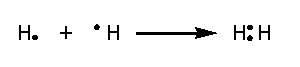
\includegraphics{dissociation/figures/h_twee.eps}
\caption{Two hydrogen atoms forming a H$_2$ molecule (Lewis structure on the right).}
\label{ch3.fig.h_twee} 
\end{figure}

If one electron is transferred from one atom to the other, which results in two oppositely charged ions, the bond is completely ionic, as in \textit{e.g.} NaCl (Figure \ref{ch3.fig.nacl}). The ions remain bound only by electrostatic interactions. 
\begin{figure}[ht]
\center
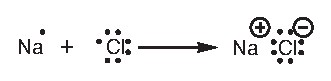
\includegraphics{dissociation/figures/nacl.eps}
\caption{A sodium and a chlorine atom forming a NaCl ``molecule''.}
\label{ch3.fig.nacl}
\end{figure}

In between these two extremes is the polar bond, which possesses mixed covalent and ionic character. Hydrogenfluoride (HF) is such a molecule (Figure \ref{ch3.fig.hf}). Although hydrogen and fluorine share electrons the electron pair will be located more on the fluorine than on the hydrogen atom, due to the higher electronegativity of fluorine.
\begin{figure}[ht]
\center
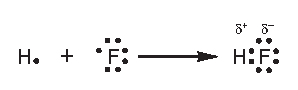
\includegraphics{dissociation/figures/hf.eps}
\caption{A hydrogen and a fluorine atom forming a HF molecule.}
\label{ch3.fig.hf}
\end{figure}

A more recently defined type of chemical bond is the charge shift bond \cite{cs1,cs2}.
\begin{figure}[h]
\center
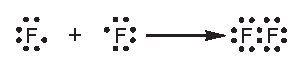
\includegraphics{dissociation/figures/f_twee.eps}
\caption{Two fluorine atoms forming a F$_2$ molecule.}
\label{ch3.fig.f_twee} 
\end{figure}
 An example of such a bond is found in fluorine (F$_2$)  (Figure \ref{ch3.fig.f_twee}). Although both fluorine atoms in F$_2$, like in H$_2$ (Figure \ref{ch3.fig.h_twee}), possess a noble gas configuration, the bond exhibits fundamental differences with H$_2$, as will be discussed in the next section.

The dissociation of polar bonds is studied with the Valence Bond method, in which the wave function can be expressed in covalent and ionic structures\footnote{See reference \cite{interpret} for a discussion on the assumed equivalence of Lewis and Valence Bond structures.}. The central question in this chapter is: How does the dissociation change when the parameters influencing the bond are changed? These parameters include internal factors, like the atoms taking part in the bond and the functional groups attached to them, and external factors, like the surrounding medium. 

To obtain answers to this question, the dissociation pathway of several polar bonds with different polarity and in different media, \textit{viz.} vacuum and water, will be studied.  The set of molecules consists of chloromethane (\textbf{1}), which possesses a typical polar C--Cl bond, \textit{tert}-butylchloride (\textbf{2}) and their silicon analogues chlorosilane (\textbf{3}) and trimethylsilylchloride (\textbf{4}) (Figure \ref{ch3.fig.compounds}).  
\begin{figure}[htbp]
\begin{center}
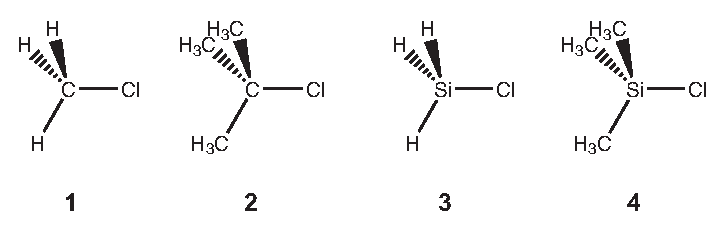
\includegraphics{dissociation/figures/compounds.eps}
\end{center}
\caption{Chloromethane (CH$_3$Cl, \textbf{1}), \textit{tert}-butylchloride
(C(CH$_3$)$_3$Cl, \textbf{2}), chlorosilane (SiH$_3$Cl, \textbf{3}) and trimethylsilanechloride
(Si(CH$_3$)$_3$Cl, \textbf{4})}
\label{ch3.fig.compounds}
\end{figure} 
The bond that will be broken is the C/Si--Cl bond.  The silicon analogues have been selected because silicon has a much lower electronegativity than carbon (compare the Pauling electronegativity of 1.90 for silicon with 2.55 for carbon \cite{handbook}). The influence this difference may have on the dissociation behavior of carbon and silicon compounds is analyzed. Furthermore, the influence of the difference between hydrogen atoms and methyl-groups on the dissocation will be compared. Methyl-groups exert an electron donating character \cite{mcmurry}, compared to hydrogen. Besides, the methyl-hydrogens might exert an effect on the dissociation process through hyperconjugation \cite{march}, not present in the hydrogen substituted compounds. Orbitals on the C--H bonds of the methyl-groups, which are several bond lengths separated from the central atom, may still have an influence on the atom, and hence on the dissociation behavior. 

The alteration of the dissociation behavior by different surrounding media will be investigated using calculations performed with the Polarizable Continuum Model (PCM) \cite{pcm1,pcm2} which accounts for solvation effects in its simplest form: the solvent is only represented as a homogeneous medium that is characterized by its dielectric constant without further explicit molecular interactions between the solvent molecules and the solute. 

The Valence Bond wave functions used to describe the dissociation behavior of these molecules contain the three structures presented in Figure \ref{ch3.fig.structures}.
\begin{figure}[htbp]
\begin{center}
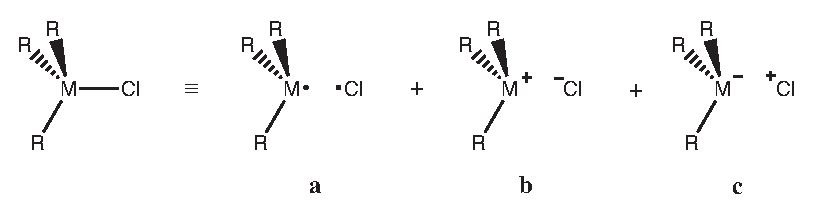
\includegraphics{dissociation/figures/structures.eps}
\end{center}
\caption{The Valence Bond structures, a covalent (\textbf{a}) and two ionic (\textbf{b} and \textbf{c}) structures (M=C or Si; R=H or CH$_3$).}
\label{ch3.fig.structures}
\end{figure}
An indication of the polarity of the bond is given by weights attributed to the structures \cite{coulson}. 

For all four compounds dissociation energies from prior VB calculations are available. Lauvergnat \textit{et al.} \cite{lauvergnat} performed VBSCF \cite{vbscf1,vbscf2} and BOVB \cite{bovb1,bovb2,bovb3} calculations on \textbf{1} and \textbf{3} in the gas phase. They concluded that BOVB is necessary to obtain a dissociation energy that is close to the experimental value (334.3 kJ/mol (BOVB) \textit{vs} 365.3 kJ/mol (experimental) for \textbf{1} and 425.5 kJ/mol (BOVB) \textit{vs} 463.2 kJ/mol (experimental) for \textbf{3}), but that VBSCF calculations sufficed to obtain qualitatively correct results.  Song \textit{et al.} \cite{song} have performed test calculations with VB in conjunction with PCM, to which they refer as VBPCM, on \textit{tert}-butylchloride (\textbf{2}) with frozen C--H bond orbitals. The latter study confirmed the heterolytic dissociation of \textbf{2} in water as a solvent. Su \textit{et al.} \cite{psu} have investigated \textbf{2} and \textbf{4} in the gas phase and with VBPCM. They have concluded that the C--Cl and Si--Cl bonds are of different natures. While C--Cl is considered to be a covalent bond, Su \textit{et al.} consider Si--Cl to be of the category of charge shift bonds. The reasoning behind this is the significantly higher resonance energy between the covalent and ionic structure in the silicon case. Our results will further extend the study of the dissociation of polar and charge shift bonds; a systematic comparison of bond dissociation in the selected compounds \textbf{1}-\textbf{4} and the influences here upon will be given.

The research is split-up in four parts.  In the first part, Valence Bond results of the dissociation of a purely covalent (H$_2$) and a purely ionic (NaCl) compound in the gas phase will be presented to illustrate the differences between the two extremes in dissociation.
Secondly, compounds \textbf{1}-\textbf{4} are investigated in the gas phase using Valence Bond theory. Thirdly, the effect of water as a solvent on the dissociation pathways of these compounds is analyzed with PCM. Finally, it will be shown that freezing of orbitals may inadvertently affect the results of the calculation. This effect is linked to hyperconjugation.

\section{Dissociation of H$_2$ and NaCl in the Gas Phase}

In the H$_2$ molecule, both hydrogen atoms contribute one electron to the bond. The two electrons can be arranged in four ways, expressed in the three Lewis structures:
\begin{equation}
\nonumber
\mathrm{H-H\ \ \equiv \ \ H^{\bullet}\ \ H^{\bullet}\ \ +\ \ H^{+}\ \ H^{-}\ \ +\ \ H^{-}\ \ H^{+}}.
\end{equation}
Both electrons can be located on their individual atoms ($\mathrm{H^{\bullet}\ \ H^{\bullet}}$) or both electrons can be located on one of the hydrogen atoms ($\mathrm{H^{+}\ \ H^{-}}$ and $\mathrm{H^{-}\ \ H^{+}}$). To analyze the dissociation of the H$_2$ bond theoretically, it is expressed in the three VB structures:
\begin{equation}
\nonumber
\Psi_{\mathrm{H_2}} = c_1\cdot [\mathrm{H}^\bullet \mathrm{H}^\bullet] + c_2 \cdot [\mathrm{H}^{+}\mathrm{H}^{-}] + c_3 \cdot [\mathrm{H}^{-}\mathrm{H}^{+}]. 
\end{equation}
Energies for the total wave function and the structures separately are calculated at different interatomic distances. Because $[\mathrm{H}^{+}\mathrm{H}^{-}]$ and $[\mathrm{H}^{-}\mathrm{H}^{+}]$ are equivalent their corresponding coefficients will be equal ($c_2 = c_3$).  

In Figure \ref{ch3.fig.h2_c} the dissociation path for H$_2$ is shown. The total energy curve ($E_\mathrm{tot}$) and the energy curves of the covalent ($E_\mathrm{cov}$) and ionic ($E_\mathrm{ion}$) structures separately are presented. 
\begin{figure}[htbp]
\begin{center}
\includegraphics[scale=0.6]{dissociation/figures/h2_g.eps}
\end{center}
\caption{The dissociation curve of H$_2$ in the gas phase. $E_\mathrm{tot}$ is the total VB energy, $E_\mathrm{cov}$  and $E_\mathrm{ion}$ are the energies of the covalent $[\mathrm{H^\bullet H^\bullet}]$ and ionic $[\mathrm{H^{+}H^{-}}]$ structures separately.}
\label{ch3.fig.h2_c}
\end{figure}
The total and covalent curves practically coincide over the whole range. This indicates the covalent character of the bond in H$_2$. For the covalent structure the weight is at least 0.8 over the whole dissociation range.

Typical for the ionic and covalent curves is that they are easily distinguishable by their shape, at least in the curves presented here. The value of $E_\mathrm{ion}$ increases with increasing bonding distance from the minimum in energy to higher distances. In the covalent curves the increase in $E_\mathrm{cov}$ from the minimum in energy going to larger distances stops at distances roughly varying from 2.5 to 4.0 \AA\ in these cases. An explanation for the sustained increasing character of the ionic curves, not seen in the covalent or neutral curves, can be found in electrostatics (Coulomb attraction): when two oppositely charged bodies, in this case atoms or molecular fragments, are separated, the potential energy increases inversely proportional to the separation distance.

In analogy with $\Psi_{\mathrm{H_2}}$, a three structure VB wave function for NaCl is constructed:
\begin{equation}
\nonumber
\Psi_{\mathrm{NaCl}} = c_1\cdot [\mathrm{Na}^\bullet \mathrm{Cl}^\bullet] + c_2 \cdot [\mathrm{Na}^{+}\mathrm{Cl}^{-}] + c_3 \cdot [\mathrm{Na}^{-}\mathrm{Cl}^{+}]. 
\end{equation}
Dissociation curves for $\Psi_{\mathrm{NaCl}}$ are presented in Figure \ref{ch3.fig.nacl_c}.
\begin{figure}[hbtp]
\begin{center}
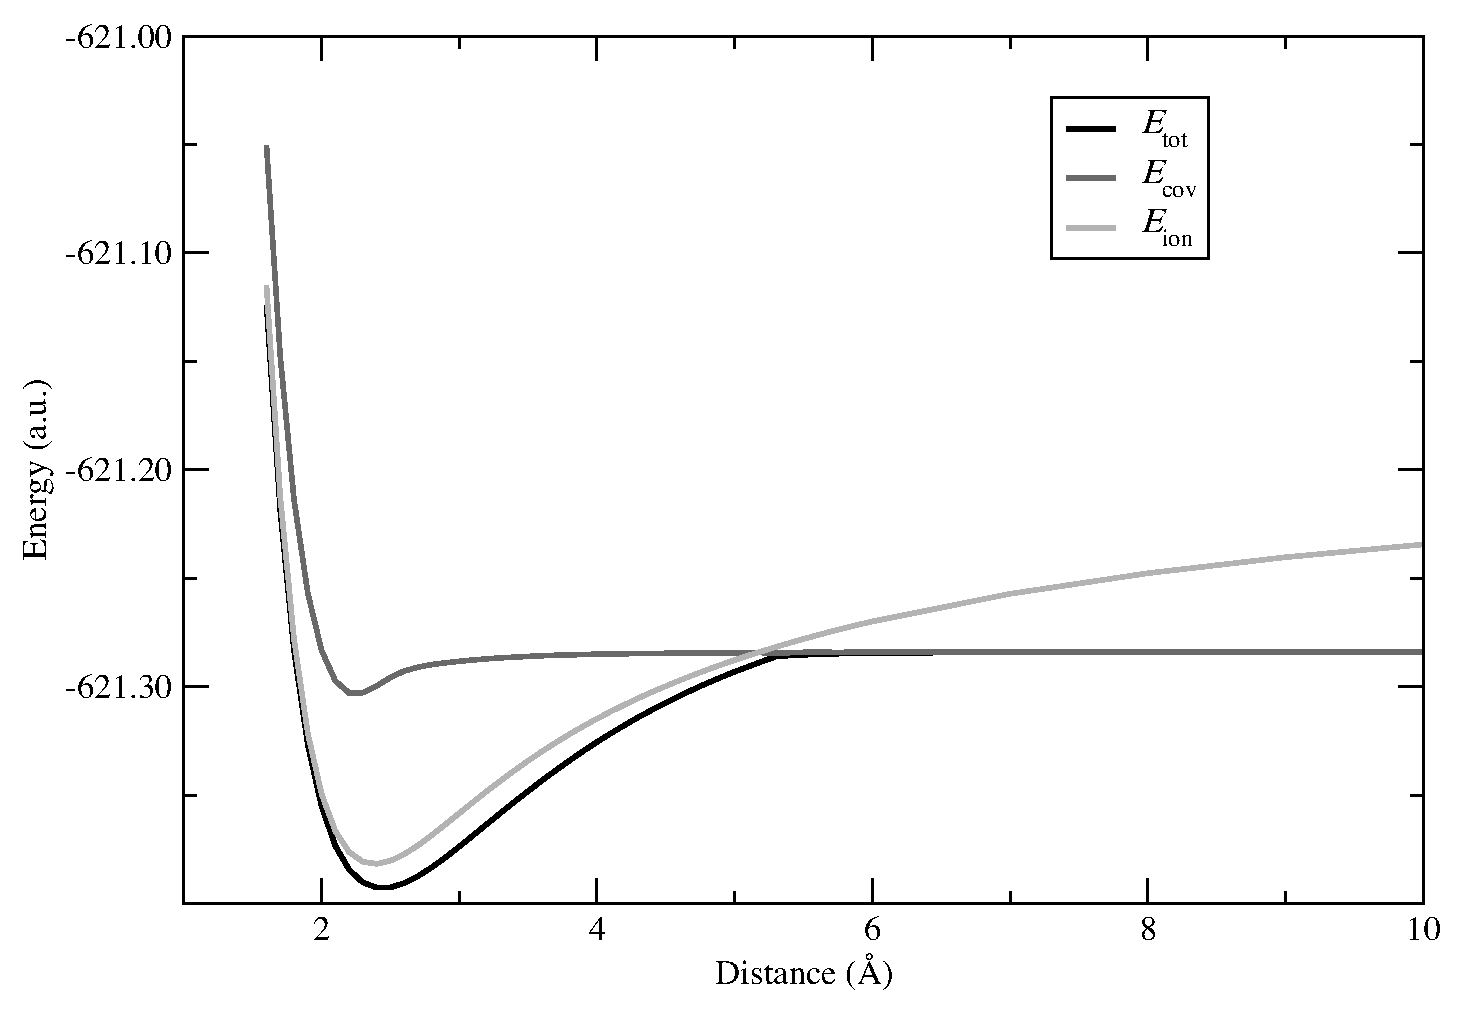
\includegraphics[scale=0.6]{dissociation/figures/nacl_g.eps}
\end{center}
\caption{The dissociation curve of the NaCl ``molecule'' in the gas phase. $E_\mathrm{tot}$ is the total VB energy, $E_\mathrm{cov}$  and $E_\mathrm{ion}$ are the energies of the covalent $[\mathrm{Na^\bullet Cl^\bullet}]$ and ionic $[\mathrm{Na^{+}Cl^{-}}]$ structures separately.}
\label{ch3.fig.nacl_c}
\end{figure}
The curve for the $[\mathrm{Na}^{-}\mathrm{Cl}^{+}]$ structure has been omitted, because its energy is approximately 0.5 a.u. higher than for the other two structures over the whole range and its contribution to the wave function is negligible ($c_3 \approx 0$). Nevertheless, it is included in $\Psi_{\mathrm{NaCl}}$ to keep the general expression of the wave functions, \textit{i.e.} built from three structures, equal for all molecules in this chapter:
\begin{equation}
\nonumber
\Psi_{\mathrm{AB}} = c_1\cdot [\mathrm{A}^\bullet \mathrm{B}^\bullet] + c_2 \cdot [\mathrm{A}^{+}\mathrm{B}^{-}] 
+ c_3 \cdot [\mathrm{A}^{-}\mathrm{B}^{+}],
\end{equation}
in which $\mathrm{A}$ and $\mathrm{B}$ can be atoms or molecular fragments (structures \textbf{a}, \textbf{b} and \textbf{c} in Figure \ref{ch3.fig.structures}).

An important difference between the curves of H$_2$ and NaCl is that in the latter case the covalent and ionic curves cross. At infinite distance the atoms Na and Cl are neutral, both having an odd number of electrons (Na 11 and Cl 17). There, the covalent description prevails, characterized by the coincidence of the $E_\mathrm{tot}$ and $E_\mathrm{cov}$ curves and the weight of 1.0 for the covalent structure. At equilibrium distance (R=2.4 \AA) both atoms roughly have a noble gas configuration (Na$^{+}$ = [Ne] and Cl$^{-}$ = [Ar]). At that point the $[\mathrm{Na}^{+}\mathrm{Cl}^{-}]$ structure forms the bonding picture, indicated by the small difference between $E_\mathrm{tot}$ and $E_\mathrm{ion}$ and its high weight of 0.7. In between those two points lies the crossing of the covalent and ionic curves, which occurs around 5.2 \AA. Although the energies for both separate structures are the same, the difference in charge distribution is large: in the covalent case the atoms are neutral, while in the ionic case sodium is positively charged and chlorine negatively charged. In a VB calculation with both structures the weight of the ionic structure is almost 0.9 at the crossing. At larger distances the weight of the ionic structure rapidly decreases to zero.

Another difference is the shape of the curves for the total energy ($E_\mathrm{tot}$): the steady increasing character for NaCl between 2.4 and 5.2 \AA, caused by the relative importance of the ionic structure, is absent in the curve for H$_2$, which rises quite rapidly to the energy level of two separate hydrogen atoms between 0.8 and roughly 2.5 \AA. So, it is expected that for bonds with ionic character, the total energy curve will exhibit more ``Coulombic character'' compared to covalent bonds. 

For both molecular systems, the total energy curves coincides with either the covalent curve (H$_2$) or the ionic curve (NaCl) around the equilibrium geometry. In between these extremes are those molecules for which the total energy curve does not coincide with a particular single structure curve. These molecules have a high resonance energy, being the energy difference between the total energy and the energy of the most stable structure in the equilibrium geometry. Those are examples of the charge shift category \cite{cs1,cs2}.

In the following section, the shapes and positions of the curves for \textbf{1}-\textbf{4} in the gas phase will be compared with each other and with H$_2$ and NaCl (the two examples mentioned above).

\section{\label{ch3.sec.gasphase}Gas Phase Dissociation of C/Si-Cl Bonds}

\subsection{Methods}

Twenty-two points on the dissociation path have been calculated with fixed lengths for the \mbox{M--Cl} bond (step \textit{1} in Figure \ref{ch3.fig.scheme1}). The other bond lengths and bond angles were optimized in $C_\mathrm{3v}$ symmetry at the \mbox{GVB/6-31G*} level \cite{gvb1,gvb2,gvb3,gvb4}, in which the \mbox{M--Cl} $\sigma$ and \mbox{M--Cl} $\sigma^{*}$ bonds were correlated.
\begin{figure}[ht]
\begin{center}
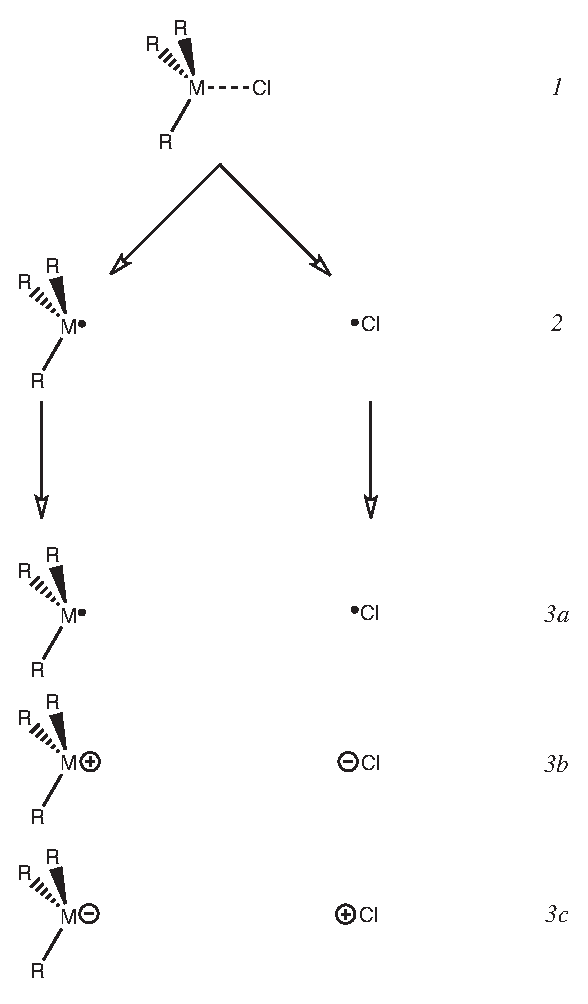
\includegraphics{dissociation/figures/scheme1.eps}
\end{center}
\caption{The three steps to generate dissociation curves: \textit{1.} Geometry optimization at fixed M--Cl (dashed) bonds. \textit{2.} Generation of start-up orbitals on radical fragments. \textit{3.} Valence Bond calculations on the three Lewis structures separately (\textit{3a}, \textit{3b} and \textit{3c}) and together (\textit{3a} + \textit{3b} + \textit{3c}).} 
\label{ch3.fig.scheme1}
\end{figure}
After these geometry optimizations startup orbitals were generated on the R$_3$M$^{\bullet}$ and Cl$^{\bullet}$ fragments separately at the \mbox{RHF/6-31G*} level (step \textit{2} in Figure \ref{ch3.fig.scheme1}).  With these orbitals the Valence Bond wave functions for the covalent (\textit{3a}), both ionic (\textit{3b} and \textit{3c}) Lewis structures and the superposition of \textit{3a}, \textit{3b} and \textit{3c} were constructed. The valence orbitals were optimized at the \mbox{VBSCF/6-31G*} level \cite{vbscf1,vbscf2}, while the core orbitals were frozen at their \mbox{RHF/6-31G*} levels.
Through the use of the local VBSCF model the orbitals were optimized on both the R$_3$M and Cl fragments separately; basis functions of the other fragment were not allowed to mix in, keeping the orbitals expressed in basis functions of a single fragment. All calculations presented here were performed with TURTLE \cite{turtle} as implemented in GAMESS-UK \cite{gamess}.

\subsection{Results and Discussion}

The optimal M--Cl bond lengths ($R_\mathrm{eq}$) and the corresponding dissociation energies ($E_\mathrm{dis}$) are shown in Table \ref{ch3.tab.optimal}. $E_\mathrm{dis}$ is the difference between the lowest energy (at equilibrium) and the energy at 10 \AA. The lowest VB energy and the optimal VB M--Cl bond lengths are obtained by a three-point fit through the three lowest points around the equilibrium. Next to our $E_\mathrm{dis}$ values, the corresponding values from literature and the experimental values \cite{lauvergnat,psu} are shown. 
\begin{table}[htp]
\center
\caption{The VB dissociation energy $E_\mathrm{dis}$ (literature data \cite{lauvergnat,psu} between parentheses) and optimal M--Cl bond lengths.}
\begin{tabular}{|l|c|c|c|c|} 
\hline
Compound & \multicolumn{3}{c|}{$E_\mathrm{dis}$ (kJ/mol)} & $R_\mathrm{eq}$ (\AA)\\
&\multicolumn{1}{c}{ours} & \multicolumn{1}{c}{lit.} & \multicolumn{1}{c|}{exp.} & (M--Cl length) \\ 
\hline
CH$_3$Cl (\textbf{1})& 260.6 & 255.6 & 365.3 & 1.893 \\
C(CH$_3$)$_3$Cl (\textbf{2}) & 251.4 & 245.6 & 360.7 & 1.935 \\
SiH$_3$Cl (\textbf{3})& 334.8 & 331.1 & 463.2 & 2.154 \\
Si(CH$_3$)$_3$Cl (\textbf{4}) & 370.8 & n/a & n/a & 2.174 \\
\hline
\end{tabular}
\label{ch3.tab.optimal}
\end{table}
Our calculated dissociation energies for \textbf{1}, \textbf{2} and \textbf{3} are in good agreement with earlier reported values at the VBSCF/6-31G* level of theory \cite{lauvergnat, psu}. As mentioned earlier, Lauvergnat \textit{et al.} \cite{lauvergnat} concluded that BOVB produces dissociation energies that are close to the experimental value, but that VBSCF calculations suffice to obtain qualitatively correct results. Song \textit{et al.} \cite{song} have found the dissociation energy for \textit{tert}-butylchloride (\textbf{2}) to be \textit{ca.} 234 kJ/mol at the VBSCF/6-31G level of theory, which is about 17 kJ/mol lower than our value. This is presumably due to the fact that they have used frozen C--H bond orbitals as will be discussed later.

For \textit{tert}-butylchloride (\textbf{2}) the dissociation energy is 9.2 kJ/mol lower than for chloromethane (\textbf{1}). For trimethylsilylchloride (\textbf{4}) it is 36.0 kJ/mol higher than for chlorosilane (\textbf{3}).

The dissociation curves of \textbf{1}-\textbf{4} are shown in Figures \ref{ch3.fig.ch3cl}, \ref{ch3.fig.c4h9cl}, \ref{ch3.fig.sih3cl} and \ref{ch3.fig.c3h9sicl}. All Figures consist of three curves in the gas phase: the total VB energy ($E_\mathrm{tot}$), the energy of the covalent structure \textbf{3a} ($E_\mathrm{cov}$) and the energy of ionic structure \textbf{3b} ($E_\mathrm{ion}$), which corresponds to R$_3$M$^{+}$ and Cl$^{-}$. The curve for R$_3$M$^{-}$ and Cl$^{+}$ (the other ionic structure \textbf{3c}) has been omitted, since the energy for \textbf{3c} was \textit{ca.} 0.3 - 0.5 a.u. higher than for the other structures over the whole range and its contribution to the wave function proved to be small.

Chloromethane (\textbf{1}; Figure \ref{ch3.fig.ch3cl}) shows covalent bond character over the whole range. 
\begin{figure}[htbp]
\begin{center}
\includegraphics[scale=0.55]{dissociation/figures/ch3cl_g.eps}
\end{center}
\caption{The dissociation curve of chloromethane (CH$_3$Cl; \textbf{1}) in the gas phase. $E_\mathrm{tot}$ is the total VB energy. $E_\mathrm{cov}$ is the energy of structure \textbf{a} and $E_\mathrm{ion}$ is the energy of structure \textbf{b} separately.}
\label{ch3.fig.ch3cl}
\end{figure}
\begin{figure}[hbtp]
\begin{center}
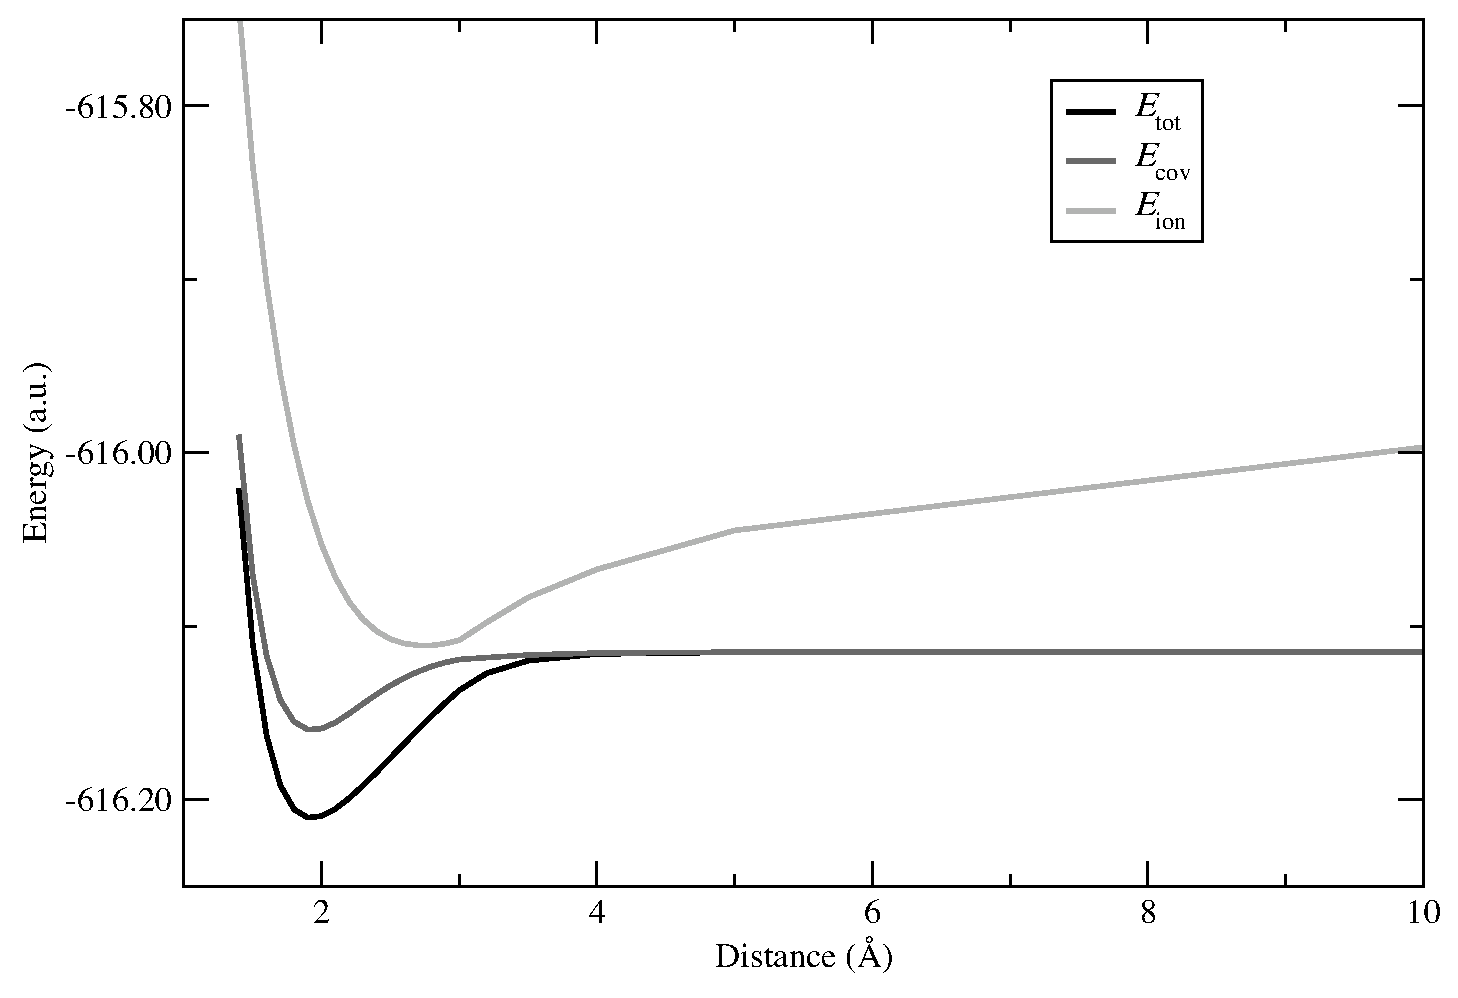
\includegraphics[scale=0.55]{dissociation/figures/c4h9cl_g.eps}
\end{center}
\caption{The dissociation curve of \textit{tert}-butylchloride (C(CH$_3$)$_3$Cl; \textbf{2}) in the gas phase. $E_\mathrm{tot}$ is the total VB energy. $E_\mathrm{cov}$ is the energy of structure \textbf{a} and $E_\mathrm{ion}$ is the energy of structure \textbf{b} separately. }
\label{ch3.fig.c4h9cl}
\end{figure}
\begin{figure}[htbp]
\begin{center}
\includegraphics[scale=0.55]{dissociation/figures/sih3cl_g.eps}
\end{center}
\caption{The dissociation curve of chlorosilane (SiH$_3$Cl; \textbf{3}) in the gas phase. $E_\mathrm{tot}$ is the total VB energy. $E_\mathrm{cov}$ is the energy of structure \textbf{a} and $E_\mathrm{ion}$ is the energy of structure \textbf{b} separately.}
\label{ch3.fig.sih3cl}
\end{figure}
\begin{figure}[hbtp]
\begin{center}
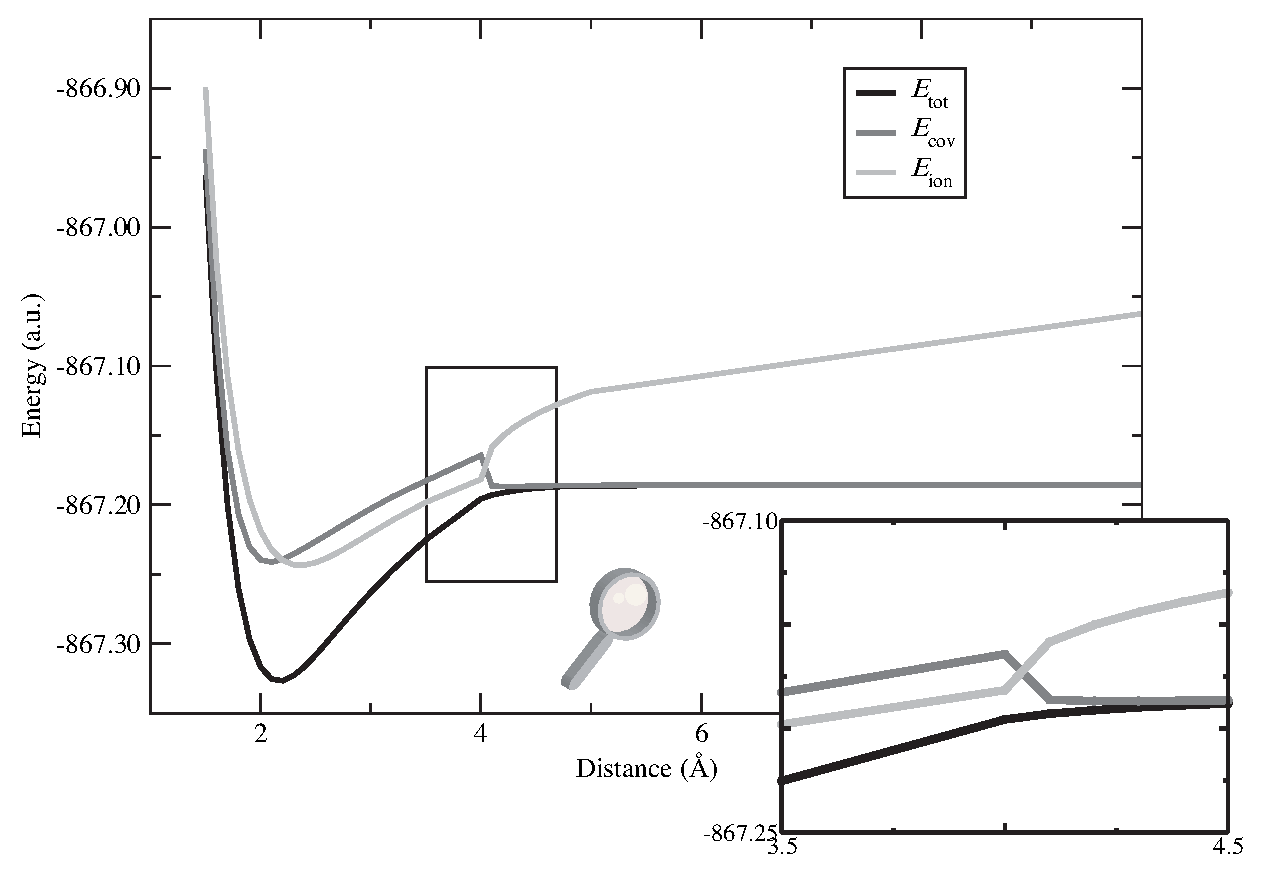
\includegraphics[scale=0.70]{dissociation/figures/c3h9sicl_g.eps}
\end{center}
\caption{The dissociation curve of trimethylsilylchloride (Si(CH$_3$)$_3$Cl; \textbf{4}) in the gas phase. $E_\mathrm{tot}$ is the total VB energy. $E_\mathrm{cov}$ is the energy of structure \textbf{a} and $E_\mathrm{ion}$ is the energy of structure \textbf{b} separately. }
\label{ch3.fig.c3h9sicl}
\end{figure}
The weight of the covalent structure is 0.67 at equilibrium distance and higher for longer distances. The bond character for \textit{tert}-butylchloride (\textbf{2}; Figure \ref{ch3.fig.c4h9cl}) is also covalent, because the weight for the covalent structure is at least 0.66 over the whole range of the curve.
In the chlorosilane (\textbf{3}) case (Figure \ref{ch3.fig.sih3cl}) the bonding energy is 74.2 kJ/mol higher than in the chloromethane (\textbf{1}) case, indicating that the Si--Cl bond is much stronger than the C--Cl bond. 

Moreover, the bond between silicon and chlorine can be considered to be of the charge shift type: at the equilibrium geometry the $E_\mathrm{cov}$ and $E_\mathrm{ion}$ values are almost equal as are the weights for the covalent and ionic structures. In contrast to both C--Cl bonds the energy minimum for the ionic structure lies close to the covalent and total minima.  

For trimethylsilylchloride (\textbf{4}; Figure \ref{ch3.fig.c3h9sicl}) the Coulombic character is more pronounced. From 2 to 4.1 \AA\  the ionic curve ($E_\mathrm{ion}$) lies below the covalent curve ($E_\mathrm{cov}$). The weight of the ionic structure is higher than that of the covalent structure between 2.3 and 4.1 \AA, which is in line with the expectation that this bond possesses a higher ionic character. Still, the bonds in trimethylsilylchloride (\textbf{4}) and NaCl are quite different, because for NaCl the ionic and total curve almost coincide, while for \textbf{4} this is not the case, although the ionic curve lies lower in energy than the covalent curve near the equilibrium distance. At large distance this situation is reversed (compare Figure \ref{ch3.fig.nacl_c} with Figure \ref{ch3.fig.c3h9sicl}). Another difference between the curves of \textbf{4} and NaCl is that for NaCl there is only one crossing of the ionic and covalent curves, whereas there are two for \textbf{4}. The crossing of \textbf{4} at short distance is not accompanied by any kind of barrier, because the geometry does not change drastically. At distances below the Si--Cl equilibrium bond distance the negative charge cloud on the chlorine atom starts to overlap with the positive Si(CH$_3$)$_3$ fragment. This stabilizes the neutral covalent structure, which results in a lower value for $E_\mathrm{cov}$ than for $E_\mathrm{ion}$. 

Regarding the shape, the total energy for \textbf{4} increases more steadily than for \textbf{2}, showing more Coulombic character. This is because from the equilibrium distance to the crossing, the ionic curve lies below the covalent curve as in the case of NaCl. In the other cases the covalent curve lies below the ionic curve over the whole range.

An intriguing feature in this figure, absent in those for the other three molecules, is the barrier in the covalent curve ($E_\mathrm{cov}$) at 4.0 \AA. This situation occurs near the crossing of the covalent and the ionic curve. The reason for this crossing is that the geometry at 4.0 \AA\ is completely different from that at 4.1 \AA. At 4.0 \AA\ the bond is ionic and hence the trimethylsilyl fragment is cation-like in which the silicon and the three carbon atoms are nearly coplanar after geometry optimization (Figure \ref{ch3.fig.crossing}(a)). This geometry is unfavorable for the covalent structure alone, reflected in the high energy.  In contrast, at 4.1 \AA\  the bond is covalent and the trimethylsilyl is radical-like, in which the silicon and the three carbon atoms form a tetrahedral structure (Figure \ref{ch3.fig.crossing}(b)), resulting in a lower covalent structure energy. 
\begin{figure}[htbp]
\center
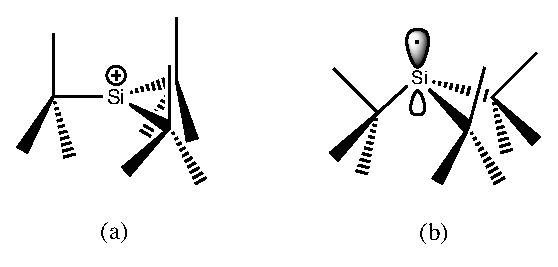
\includegraphics[scale=1.0]{dissociation/figures/crossing.eps}
\caption{The cation-like structure with coplanar silicon and methyl carbon atoms (a) and the radical-like tetrahedral structure (b).}
\label{ch3.fig.crossing}
\end{figure}
The total energy curve ($E_\mathrm{tot}$) does not show any irregularities.  The wave function changes drastically in character at this point. This compound follows the dissociation path of the ionic structure at short distances and that of the covalent structure at longer distances. 

A comparison of the hydrogen and methyl substituted molecules suggests that methyl substitution has an energy lowering effect on the $E_\mathrm{ion}$ with respect to $E_\mathrm{cov}$. In the silicon case (\textbf{4}), the ionic curve even lies below the covalent curve between 2.3 and 4.1 \AA. The reason for this lowering might be the effect of hyperconjugation, as will be discussed later.

\section{\label{ch3.sec.solv}Solvation Effects}

\subsection{Methods}

In the Polarizable Continuum Model (PCM) the solvent is, as already stated in the introduction, only represented as a homogeneous medium that is characterized by its dielectric constant. No further explicit molecular interactions between the solvent molecules and the solute are taken into account. For example, hydrogen-bond formation is absent. The test calculations of Song \textit{et al.} show that VB can readily be extended with PCM \cite{song}. For the research presented here, the VB module TURTLE and the PCM algorithm in GAMESS-UK were linked. 

The PCM model requires a number of parameters. First of all, a dielectric constant, for which the value of water (H$_2$O, $\epsilon$=78.5) was chosen. The second parameter is the interspacing of the point charges, which was set to 30.0\degrees. The last set of parameters contains the dimensions of the spheres around the atoms. For these the van der Waals radii \cite{bondi} were taken, scaled by 1.20 (being the average of the optimal 1.15 for ions and 1.25 for neutral atoms \cite{scaling}) resulting in 1.44 \AA\  for hydrogen, 2.16 \AA\  for carbon, 2.69 \AA\ for silicon and 2.10 \AA\ for chlorine and chloride.

For each compound two points on the potential energy curve were analyzed with VB and PCM. One calculation was performed at the equilibrium distance and one at large distance (10 \AA). For the point at equilibrium distance the gas phase optimized geometries were taken. For the point at large distance the R$_3$M-fragments were optimized in two ways: once as the covalent structure (a geometry optimization on the radical R$_3$M$^\bullet$-fragments) and once as the ionic structure (a geometry optimization on the R$_3$M$^{+}$-fragments). Subsequently, the chlorine atoms were added to the R$_3$M-fragments at a distance of 10 \AA. 

\subsection{Results and Discussion}

In Table \ref{ch3.tab.solution} the VBPCM values are presented for the equilibrium distance ($E_\mathrm{R_{3}M-Cl}^\mathrm{solv}$) and for both neutrally and ionically optimized geometries at large distance, $E_\mathrm{R_{3}M^\bullet Cl^\bullet}^\mathrm{solv}$ and $E_\mathrm{R_{3}M^{+} Cl^{-}}^\mathrm{solv}$ respectively. Besides, the dissociation energy in the gas phase ($E_\mathrm{dis}$) and in solution ($E_\mathrm{dis}^\mathrm{solv}$) are shown in the last two columns.
\begin{table}[htp]
\center
\caption{The VBPCM energy at equilibrium distance ($E_\mathrm{R_{3}M-Cl}^\mathrm{solv}$), the VBPCM energies on the neutrally ($E_\mathrm{R_{3}M^\bullet Cl^\bullet}^\mathrm{solv}$) and ionically ($E_\mathrm{R_{3}M^{+} Cl^{-}}^\mathrm{solv}$) optimized geometries at long distance (10 \AA), and the dissociation energy ($E_\mathrm{dis}^\mathrm{solv}$), being the difference between the most stable long distance geometry (\textit{italics}) and the energy at equilibrium distance ($R_\mathrm{eq}$). The last column contains the dissociation energies from Table \ref{ch3.tab.optimal}. Energy values are in atomic units, except $E_\mathrm{dis}^\mathrm{solv}$ and $E_\mathrm{dis}$, which are in kJ/mol.}
\begin{tabular}{|l|c|c|c|c|c|}
\hline
\textbf{Compound} & $E_\mathrm{R_{3}M-Cl}^\mathrm{solv}$ ($E_{\mathrm{h}}$) & $E_\mathrm{R_{3}M^\bullet Cl^\bullet}^\mathrm{solv}$ ($E_{\mathrm{h}}$) & $E_\mathrm{R_{3}M^{+} Cl^{-}}^\mathrm{solv}$ ($E_{\mathrm{h}}$) & $E_\mathrm{dis}^\mathrm{solv}$&
$E_\mathrm{dis}$\\
\hline
CH$_3$Cl (\textbf{1})& --499.102825 & \textit{--499.000733} & --498.984704 & 267.8 & 260.6 \\
C(CH$_3$)$_3$Cl (\textbf{2})& --616.215745 & --616.104359 & \textit{--616.169955} & 120.1 & 251.4 \\
SiH$_3$Cl (\textbf{3})& --750.179421& --750.049131 & \textit{--750.065094} &  299.9 & 334.8 \\
Si(CH$_3$)$_3$Cl (\textbf{4})& --867.333737 & --867.187192 & \textit{--867.251939} & 214.6 & 370.8 \\
\hline
\end{tabular}
\label{ch3.tab.solution}
\end{table} 

The ionic structures are more stabilized by the polar solvent than the covalent structures. At large distance the ionic structure has a lower energy for \textbf{2}, \textbf{3} and \textbf{4}, in the polar medium. This indicates that for these molecules the dissociation changes from homolytic to heterolytic with PCM. For \textbf{1}, which contains the least polar bond, the ionic structure is stabilized, however, not enough to change the dissociation to heterolytic in the solvent model.

\section{The Frozen Orbital Approximation}

Upon comparing the ionic and covalent curves for \textit{tert}-butylchloride (\textbf{2}) shown in Figure \ref{ch3.fig.c4h9cl} with those in the article by Song \textit{et al.} \cite{song}, we have noted that in the article by Song the ionic and covalent curves cross twice, while in our curves there is no crossing between the two curves. One difference between both calculations appeared to be the use of frozen orbitals for the C--H bonds by Song, while we optimized those with the other orbitals. Therefore, the impact of the freezing of orbitals will be investigated here for \textbf{2}.

\subsection{Methods}

Two points on the C--Cl reaction coordinate were taken, one at equilibrium distance and one at \mbox{10 \AA}. The start-up orbitals for both fragments were generated with a RHF wave function with the 6-31G* basis set. For each point two sets of RHF start-up orbitals were generated: \textbf{I}) for the neutral fragments (CH$_3$)$_3$C$^\bullet$ and Cl$^\bullet$ (homolytic dissociation) and \textbf{II}) for the ions, (CH$_3$)$_3$C$^{+}$ and Cl$^{-}$ (heterolytic dissociation). Subsequently, the orbitals on the (CH$_3$)$_3$C$^\bullet$ and (CH$_3$)$_3$C$^{+}$ fragments were localized using the Pipek-Mezey algorithm \cite{pipek}. The localized orbitals describing the inner-shells and C--H bonds were frozen during the subsequent VB calculations, as were the core orbitals of chlorine.  For the PCM solvation model the same parameters as in Section \ref{ch3.sec.solv} were used.

\subsection{\label{ch3.sec.res.freez}Results and Discussion}

The total VB energies for calculations with start-up sets \textbf{I} and \textbf{II}, together with the total VB energies from Section \ref{ch3.sec.solv} ($E_\mathrm{free}$) are given in Table \ref{ch3.tab.frozen}. 
\begin{table}[htp]
\center
\caption{VB energies without frozen C--H bonds ($E_\mathrm{free}$), with frozen C--H bonds based on
start-up set \textbf{I} ($E_\mathrm{froz-\textbf{I}}$) and with frozen C--H bonds based on start-up set \textbf{II}
($E_\mathrm{froz-\textbf{II}}$) at equilibrium distance ($R_\mathrm{eq}$) and at 10.0 \AA\ ($R_{10.0 \AA}$),
both in the gas phase and in solution (in $E_\mathrm{h}$). The dissociation energy in gas phase ($E_\mathrm{dis}$) and in solution ($E_\mathrm{dis}^\mathrm{solv}$) both in kJ/mol.}
\center
\begin{tabular}{|c|cc|cc|c|c|}
\hline
&\multicolumn{2}{c|}{$R_\mathrm{eq}$}&\multicolumn{2}{c|}{$R_{10.0 \AA}$} & $E_\mathrm{dis}$ & $E_\mathrm{dis}^\mathrm{solv}$ \\
\textbf{Energy} & gas & solv & gas & solv &&\\
\hline
$E_\mathrm{free}$ & {--616.209425} & {--616.219424} & {--616.114690} & {--616.118828} & 248.7 & 264.1 \\
$E_\mathrm{froz-\textbf{I}}$& {--616.207855} & {--616.216662} & {--616.114690} & {--616.118702} & 244.6 & 257.2 \\
$E_\mathrm{froz-\textbf{II}}$& {--616.184354} & {--616.200073} & {--616.083892} & {--616.092473} & 263.8 & 282.5 \\ \hline
\end{tabular}
\label{ch3.tab.frozen}
\end{table}

The frozen orbital set $E_{\mathrm{froz}-\textbf{I}}$ gives a qualitatively correct description of the dissociation process, both in the gas phase and in solution, although the dissociation energy in solution is slightly lower than for the free C--H orbitals. The dissociation energy in the gas phase and in solution for the second set of frozen orbitals ($E_{\mathrm{froz}-\textbf{II}}$) is much higher than for free C--H orbitals. This indicates that the way these frozen C--H orbitals are calculated has a significant influence on the dissociation energy. Therefore, these bonds are not mere spectators: they play a vital role in the dissociation process. In the next section, the interaction of the C--H bonds with the central carbon atom, linked to hyperconjugation \cite{march,mcmurry}, is investigated in more detail.
 
\subsection{Hyperconjugation}

When the C--H bond orbitals are frozen, the interactions between them and the $p$ orbital on the central carbon atom are absent in the wave function (Figure \ref{ch3.fig.hyperconjugation}).
\begin{figure}[ht]
\center
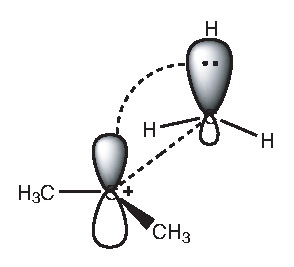
\includegraphics{dissociation/figures/hyperconj.eps}
\caption{The hyperconjugation effect: the $p$ orbital on the central carbon atom has interaction with the neighboring C--H orbital.}
\label{ch3.fig.hyperconjugation}
\end{figure}

Hyperconjugation can be included or excluded from the Valence Bond wave function by applying appropriate restrictions during orbital optimization.  Calculations on the constrained $C_\mathrm{3h}$ geometries (Figure \ref{ch3.fig.c3h}) of the \textit{tert}-butylcation, the trimethylsilylcation, and of their radicals have been performed in which the empty/singly occupied $p$ orbital on the central carbon/silicon atom is constrained to remain strictly atomic in nature, thereby excluding the effect of hyperconjugation.
\begin{figure}[ht]
\center
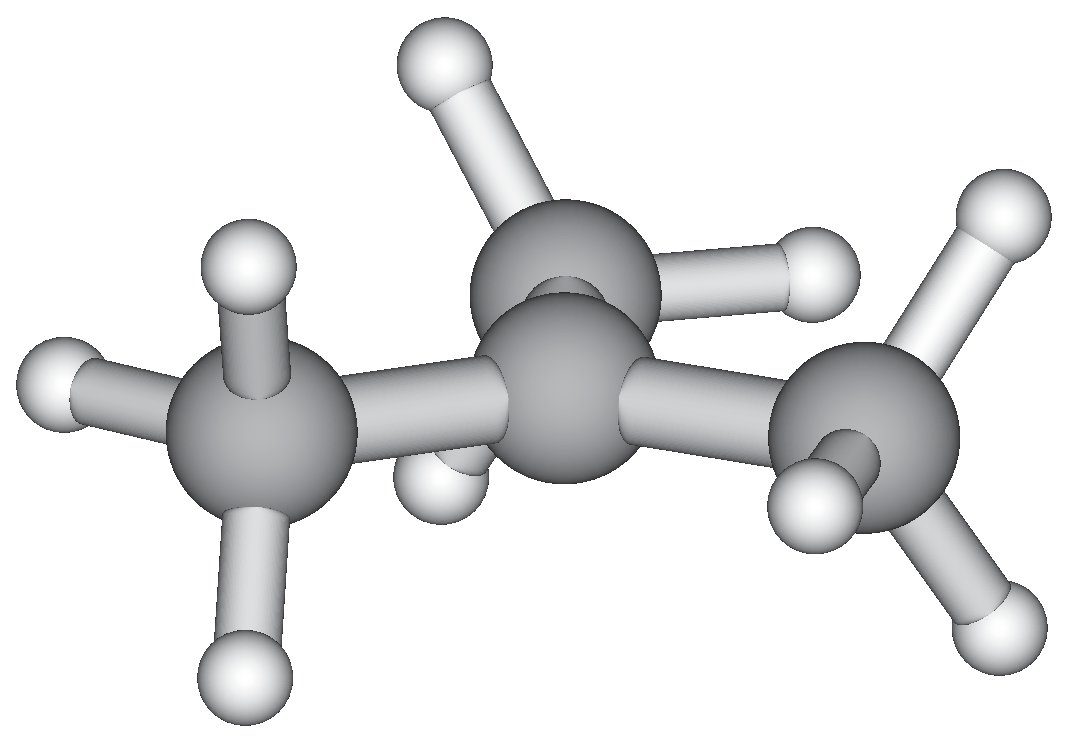
\includegraphics{dissociation/figures/c3h.eps}
\caption{Schematic representation of the \textit{tert}-butyl fragment in $C_\mathrm{3h}$ symmetry.}
\label{ch3.fig.c3h}
\end{figure}
Comparison of the energy obtained with this constrained wave function with that by an unconstrained calculation  (Hartree-Fock in this case) yields an estimate of the magnitude of the stabilization by hyperconjugation for the respective cations and radicals. 

\begin{table}[htp]
\center
\caption{Energies of the cation and radical of \textit{tert}-butyl and of the cation and the radical of trimethylsilyl obtained using a constrained VB wave function with a strictly atomic $p$ orbital ($E_\mathrm{VB-res}$) in the first column. The second column shows the Hartree-Fock energies ($E_\mathrm{HF}$) and the third column contains their difference $\Delta E$ (in kJ/mol).}
\label{ch3.tab.hyp}
\begin{tabular}{|c|c|c|c|}
\hline
\textbf{Compound} & $E_\mathrm{VB-res}$ ($E_{\mathrm{h}}$) &$E_\mathrm{HF}$ ($E_{\mathrm{h}}$)& $\Delta E$ (kJ/mol)  \\
\hline
\textit{tert}-butyl cation & -156.399322 &-156.442412&113.1  \\
\textit{tert}-butyl radical & -156.630889 &-156.661317&79.9 \\
trimethylsilyl cation & -407.509449&-407.526979&46.0 \\
trimethylsilyl radical &-407.687692&-407.704949&45.3 \\
\hline
\end{tabular}
\end{table}

From a survey of the data in Table \ref{ch3.tab.hyp} follows that the stabilization obtained for the cation and the radical by mixing of the C--H bonds with the central $p$ orbital of carbon is considerable, and substantially larger in the case of the cation than for the radical.  This further corroborates that the \textit{tert}-butyl C--H bonds of the cation differ markedly from that of the radical, as was already noted from the calculations with the different sets of frozen orbitals.  Note that for the \textit{tert}-butyl radical, the equilibrium geometry will deviate from $C_\mathrm{3h}$ symmetry, and the central $p$ orbital will rehybridize.  As a consequence of the geometric distortion and their rehybridization, the overlap between the central carbon $p$ orbital and the C--H bonds will be smaller, thus the above mentioned stabilization of 79.9 kJ/mol is an upper bound.  These calculations provide strong evidence for the large stabilizing effect that hyperconjugation exerts on the central carbon atom, and as a consequence, freezing these orbitals to describe two different reaction pathways may lead to substantial errors.  Furthermore, hyperconjugation is only important in the dissociated fragments.

For the silicon case, although a stabilization is found, it is considerably smaller than for the carbon analogue.  The trimethylsilyl cation and radical are equally stabilized.  The smaller stabilization of the trimethylsilyl fragment with respect to their carbon analogues is attributed to the more electropositive nature of silicon. Thus, hyperconjugation is less important for trimethylsilyl compounds than for the carbon analogues.

\section{Conclusions}

Both the weights and the similarity of the forms of the dissociation curves to that of H$_2$ for the C--Cl bonds of \textbf{1} and \textbf{2}, indicate that these bonds are mainly covalent.  The Si--Cl bonds are more ``Coulombic'' in nature; the shape of the dissociation curves is resembling the one of NaCl. Because neither the energy of the covalent structure nor of the ionic structure coincides with the total energy, these bonds are categorized as charge shift bonds. For \textbf{4}, the unexpected barrier in the dissociation curve for the individual covalent structure is caused by the dramatic change in geometry, due to the change in character from ionic to covalent of the wave function.  The reaction paths of the one-structure wave functions differ from that of the three-structure wave function.

Substitution of hydrogen for methyl groups does not change the C/Si--Cl bond directly, but the methyl groups exert an effect on the dissociated fragments through hyperconjugation.  The C--H bonds participate in the reaction.  Change to a medium that mimics a polar solvent (water) stabilizes the ionic curve, and may therefore change the dissociation from homo- to heterolytic, if the resulting cation is also stabilized by its electropositiveness or hyperconjugation.
 
\section*{Acknowledgement}

Part of this research was conducted in the Laboratoire de Chimie Physique, Paris XI (France) and was funded by the European Union (a Marie Curie host fellowship) and the Netherlands Organization for Scientific Research (NWO).

\bibliography{dissociation}
\bibliographystyle{../main/achemso}
